% 如果不需要调整基础信息显示, 这一部分就不需要改动, 信息填充在main.tex文件中
% 这一部分从cls文件中分离出来是为了解决链接显示的问题

%基础信息
\vspace{-1cm}
\begin{minipage}[t]{0.35\textwidth}
    \makebox[4em][s]{籍\hfill 贯}: \makebox[7em][l]{\hometown} \\
    \makebox[4em][s]{电\hfill 话}: \makebox[7em][l]{\phone} \\
    \makebox[4em][s]{学历}: \makebox[7em][l]{\education} \\
    \makebox[4em][s]{出生年月}: \makebox[7em][l]{\birthdate} \\
    \makebox[4em][s]{毕业院校}: \makebox[7em][l]{\school}\\
    \makebox[4em][s]{专业}: \makebox[7em][l]{\major} \\
\end{minipage}
\begin{minipage}[t]{0.45\textwidth}
    \makebox[2em][s]{邮\hfill 箱}: \makebox[9em][l]{\email} \\\\
    \makebox[4em][s]{个人主页}: \makebox[9em][l]{\homepage} \\\\
    \makebox[4em][s]{通讯地址}: \makebox[9em][l]{\address} \\
\end{minipage}
\begin{minipage}[t]{0.2\textwidth}
    \raisebox{-0.9\height}{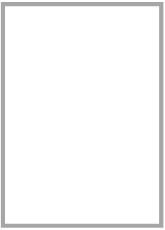
\includegraphics[width=.8\linewidth]{figures/test.png}}
\end{minipage}